\documentclass[a4paper,10pt]{article}

\usepackage{graphicx}
\usepackage[pdftex,bookmarks=true,breaklinks=true,colorlinks,linkcolor=black,filecolor=blue,urlcolor=blue,hypertexnames=false]{hyperref}

\hypersetup{
pdfauthor = {Nathan Dumont},
pdftitle = {Dwarf: A PICKit2 GUI for Linux},
pdfsubject = {Software Manual}}
%opening
\title{Dwarf: A PICKit 2 GUI for Linux}
\author{Nathan Dumont}

\begin{document}

\maketitle

\tableofcontents

\newpage
\section{License}
\begin{verbatim}
Dwarf: A PICKit 2 GUI for Linux
Copyright (C) 2009 Nathan Dumont

This program is free software: you can redistribute it and/or modify
it under the terms of the GNU General Public License as published by
the Free Software Foundation, either version 3 of the License, or
(at your option) any later version.

This program is distributed in the hope that it will be useful,
but WITHOUT ANY WARRANTY; without even the implied warranty of
MERCHANTABILITY or FITNESS FOR A PARTICULAR PURPOSE.  See the
GNU General Public License for more details.

You should have received a copy of the GNU General Public License
along with this program.  If not, see <http://www.gnu.org/licenses/>.
\end{verbatim}

\section{Revisions}
\begin{tabular}{ll}
 9-Sep-2009&Version 0.1 documentation with initial release.
\end{tabular}

\section{Introduction}
I've been using a PICKit 2 for a couple of years now, it was a brilliant advance for hobbyist PIC programmers.  However until now I've been using it from Windows in some way (usually a virtual machine running on top of Linux.)  I am about to start a major new project and decided to start from scratch on Linux and avoid the Windows hassle entirely.  I found the command line utilities for compiling (gpasm) and programming (pk2cmd) fairly easy to use, but I'm quite lazy and didn't want to bother with typing in the command every time.  Dwarf was the result of this and a few days waiting for parts to arrive.

Dwarf is a very simple PyGTK GUI for the command line utilities gpasm for compiling and pk2cmd for controlling the PICKit 2 programmer from Microchip.  The UI provides a compile button to compile PIC assembly files, a program button to program the device with a binary file, and a run and stop button to allow powering projects from the PICKit 2.  There are some basic features like age checking on the compiled and source file and PIC model checking to warn the user about possible errors.

The name Dwarf was chosen because it is a small program, and because in most literary references dwarves are closely linked with mining and therefore picks.

\section{Installation}
Dwarf has several dependencies, all of which must be installed manually first.  It requires Python installed and PyGTK, these are likely to be installed already if you are using a modern desktop Linux distribution.  I would advise that you run dwarf from the command line the first time and check for errors about python modules.

The compiler (gpasm) needs to be installed if you intend to use the program to compile source files.  You can run it without if you only intend to use it for programming.  gpasm is part of the GNU PIC Utilities package (GPUtils) and is probably available as a package for your distribution.  Otherwise check \href{http://gputils.sourceforge.net/}{http://gputils.sourceforge.net/}.

The programmer interface is done through the pk2cmd utility.  This is available from the \href{http://www.microchip.com/stellent/idcplg?IdcService=SS_GET_PAGE&nodeId=1406&dDocName=en023805&redirects=pickit2}{Microchip website}, the program is available near the bottom of the page, you need the Linux PK2CMD utility.  Follow the instructions in the tar to install the utility.

Dwarf is a single Python script, it needs the images in the \texttt{data} folder for the buttons.  Choose where you want the executable and ensure that the file \texttt{dwarf} has the execute permission and that the \texttt{data} folder is in the same directory as \texttt{dwarf}.  You can now run the program by executing \texttt{./dwarf} from a command line in the same folder as the script.

\section{Interface}
\subsection{Graphical Interface}
The user interface for Dwarf is illustrated in Figure \ref{fig:ui}

\begin{figure}[h]
 \begin{center}
  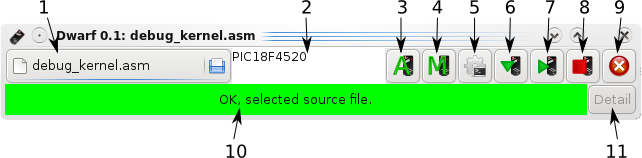
\includegraphics[width=120mm]{doc.png}
 \end{center}
 \caption{Standard GUI appearance}
 \label{fig:ui}
\end{figure}

The controls function as detailed below:\\\\
\begin{tabular}{lll}
 1&File Selector&Use this to select the assembly or HEX file.\\
 \hline
 2&Device Model&Displays the device type, manually edit for\\
 &&non-auto-detectable devices (e.g. eeproms)\\
 \hline
 3&Auto-detect&Auto detect the attached device, works for most\\
 &&PIC devices, run automatically at start\\
 \hline
 4&Manual detect&If you've selected a device type manually click\\
 &&this to check a PICKit is attached and a device\\
 &&is present, once complete the program buttons\\
 &&will be enabled.\\
 \hline
 5&Compile&This button is enabled once a source file\\
 &&(*.asm) is selected with the file selector.  It\\
 &&will compile with the default settings of \texttt{gpasm}\\
 &&in the directory that the source file is located.\\
 &&Warnings and errors are available from the\\
 &&status detail window.\\
 \hline
 6&Program the Device&Clicking this downloads the selected HEX file.\\
 &&If the file selected is an assembly file, it will\\
 &&compare the age of that file with the HEX file\\
 &&and issue a warning if you've editted the source\\
 &&since you last compiled.  If the selected file is a\\
 &&HEX file it will just program the device with\\
 &&that file.\\
 \hline
 7&Run&This powers the target from the PICKit and\\
 &&releases the MCLR line, this is useful for\\
 &&running low powered applications without an\\
 &&external source.\\
 \hline
 8&Stop&Turn off power to the target.\\
 \hline
 9&Exit&Closes Dwarf.\\
 \hline
 10&Status display&Shows the status of the last operation and brief\\
 &&error or warning messages.\\
 \hline
 11&Status details&If an operation produces detailed status output\\
 &&e.g. a compile with error messages, these are\\
 &&available in a second window which will be\\
 &&shown by clicking the Detail button.  Note that\\
 &&this window does not update automatically you\\
 &&need to close it and click detail again if you\\
 &&have performed another operation.\\
\end{tabular}

\subsection{Command Line Options}
There is currently only one command line option, the \texttt{-v} option which outputs debugging information about the commands being run.
\section{Contact Details}
If you find any bugs or want to suggest features for Dwarf you can contact me at hairymnstr@gmail.com

\end{document}
